\documentclass[tikz,border=3pt]{standalone}
\usepackage{amsmath}
\usetikzlibrary{arrows.meta,positioning,calc,fit}

\definecolor{cSlow}{HTML}{2878B5}
\definecolor{cFast}{HTML}{E67E22}
\definecolor{cCache}{HTML}{2E8B57}
\definecolor{cInk}{HTML}{263238}

\tikzset{
  flow/.style={-{Latex[length=1.8mm]},line width=0.7pt,draw=cInk},
  slowbox/.style={rounded corners=2pt,draw=cSlow,fill=cSlow!9,line width=0.85pt,
                  align=center,font=\sffamily\scriptsize,minimum height=7mm},
  fastbox/.style={rounded corners=2pt,draw=cFast,fill=cFast!10,line width=0.85pt,
                  align=center,font=\sffamily\scriptsize,minimum height=7mm},
  cachebox/.style={rounded corners=2pt,draw=cCache,fill=cCache!9,line width=0.85pt,
                   align=center,font=\sffamily\scriptsize,minimum height=8mm},
  label/.style={font=\sffamily\scriptsize\bfseries,text=cInk},
  note/.style={font=\sffamily\tiny,align=center,text=cInk!75}
}

\begin{document}
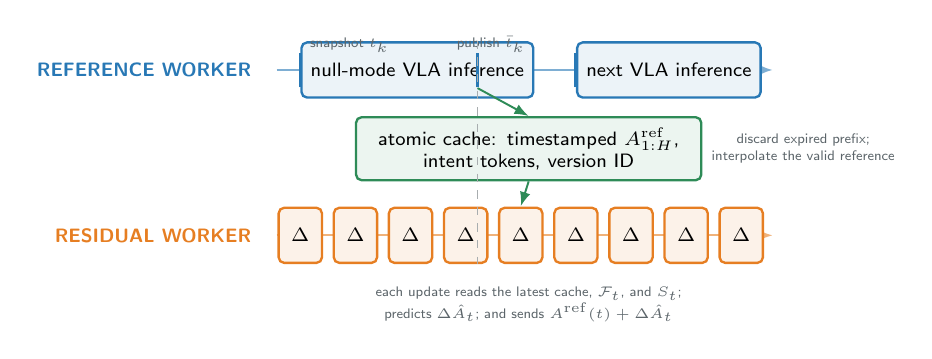
\begin{tikzpicture}[x=1cm,y=1cm]
  \node[label,anchor=east,text=cSlow] at (1.65,2.65) {REFERENCE WORKER};
  \draw[line width=0.7pt,draw=cSlow!60,-{Latex[length=1.6mm]}] (1.85,2.65) -- (8.15,2.65);
  \node[slowbox,anchor=west,minimum width=2.25cm] (infer1) at (2.15,2.65)
    {null-mode VLA inference};
  \node[slowbox,anchor=west,minimum width=2.05cm] (infer2) at (5.65,2.65)
    {next VLA inference};
  \draw[line width=1.2pt,draw=cSlow] (2.15,2.43) -- (2.15,2.87);
  \draw[line width=1.2pt,draw=cSlow] (4.40,2.43) -- (4.40,2.87);
  \draw[line width=1.2pt,draw=cSlow] (5.65,2.43) -- (5.65,2.87);
  \node[note,above=1mm of infer1.west,anchor=south west] {snapshot $t_k$};
  \node[note,above=1mm of infer1.east,anchor=south east] {publish $\bar t_k$};

  \node[cachebox,text width=4.15cm] (cache) at (5.05,1.65)
    {atomic cache: timestamped $A^{\mathrm{ref}}_{1:H}$,\\intent tokens, version ID};
  \draw[flow,draw=cCache] (4.40,2.42) -- (cache.north);
  \node[note,anchor=west] at (7.25,1.65)
    {discard expired prefix;\\interpolate the valid reference};

  \node[label,anchor=east,text=cFast] at (1.65,0.55) {RESIDUAL WORKER};
  \draw[line width=0.7pt,draw=cFast!60,-{Latex[length=1.6mm]}] (1.85,0.55) -- (8.15,0.55);
  \foreach \x in {2.15,2.85,3.55,4.25,4.95,5.65,6.35,7.05,7.75} {
    \node[fastbox,minimum width=5.5mm,inner sep=1pt] at (\x,0.55) {$\Delta$};
  }
  \draw[flow,draw=cCache] (cache.south) -- (4.95,0.92);
  \node[note,anchor=north] at (5.05,0.02)
    {each update reads the latest cache, $\mathcal F_t$, and $S_t$;\\predicts $\Delta\hat A_t$; and sends $A^{\mathrm{ref}}(t)+\Delta\hat A_t$};

  \begin{scope}
    \draw[dashed,draw=cInk!40] (4.40,3.02) -- (4.40,0.18);
  \end{scope}
\end{tikzpicture}
\end{document}
